\section{Results}
\label{sec:results}

In this section we demonstrate the utility of our novel framework on three hitherto uninvestigated questions: (i) an exact functional representation of the multi-objective trade-offs in a multi-objective navigation domain; (ii) exact sensitivity analysis of public health policies in epidemic models over the full range of infection rate parameters; and (iii) non-convex optimization of policy parameters applied to finance problems previously impossible with sample-based policy gradient techniques.

\subsection{Multi-objective Navigation}
\label{sec:results_navigation}

In this domain we consider an autonomous vehicle moving along one dimension, e.g. along the real number line. At each stage the vehicle must trade-off between moving into a potentially higher reward region and incurring a cost associated with movement. The domain is specified as follows:
\begin{itemize}
    \item {\footnotesize $ \State = \left\langle loc \right\rangle$}, where $ loc $ is the location of the vehicle.
    \item {\footnotesize $ \Action \in \left\lbrace -5.0, 0.0, 5.0 \right\rbrace $} is the amount by which vehicle moves relative to its current location.
    \item {\footnotesize $ \Transition\left( loc' | loc, a \right) = \delta \left[ loc' - (loc + a) \right] $}
    \item {\footnotesize $ \Reward\left(\vec{w}, loc, a, \mathtt{threshold} \right) = w_1 \cdot \Reward_{\mathtt{location}} + w_2 \cdot \Reward_{\mathtt{movement}} $} where, \\
    {\footnotesize 
        \abovedisplayskip=10pt
        \belowdisplayskip=0pt
        \renewcommand{\arraystretch}{1.5}
        \begin{tabular}{ll}    
            $ \Reward_{\mathtt{location}}(loc', \mathtt{threshold}) = $ &  $ $ \\
                \qquad $ \begin{cases}
                (loc' \geq \mathtt{threshold}) : & loc' \\
                \text{otherwise} : & 0.0 \\
                \end{cases} $ & $ $\\
            $ \Reward_{\mathtt{movement}}(\cdot) = -cost_{\mathtt{movement}} $ & $ $ \\                        
        \end{tabular}
    }    
\end{itemize} 

In Figure~\ref{fig:vehicle1d} we present the optimal {\footnotesize$ \Horizon = 10 $} value function for the multi-objective navigation domain with {\footnotesize $w_1 = 1.0$}, {\footnotesize $ \mathtt{threshold} = 10.0 $} and {\footnotesize$ cost_{\mathtt{movement}} = 1.0 $}. The value function shows that when the location of the vehicle is below the {\footnotesize $ \mathtt{threshold} $}, the actions of the vehicle depends on the value of {\footnotesize $ w_2 $}; large values of {\footnotesize $ w_2 $} leads to the vehicle staying in its current location, whereas at smaller values of {\footnotesize $ w_2 $}, the vehicle is likely to move towards the goal region and incur the movement cost.
%------------------------------------------------------------------------------
% Figure
\begin{figure}[h!]
    \centering
    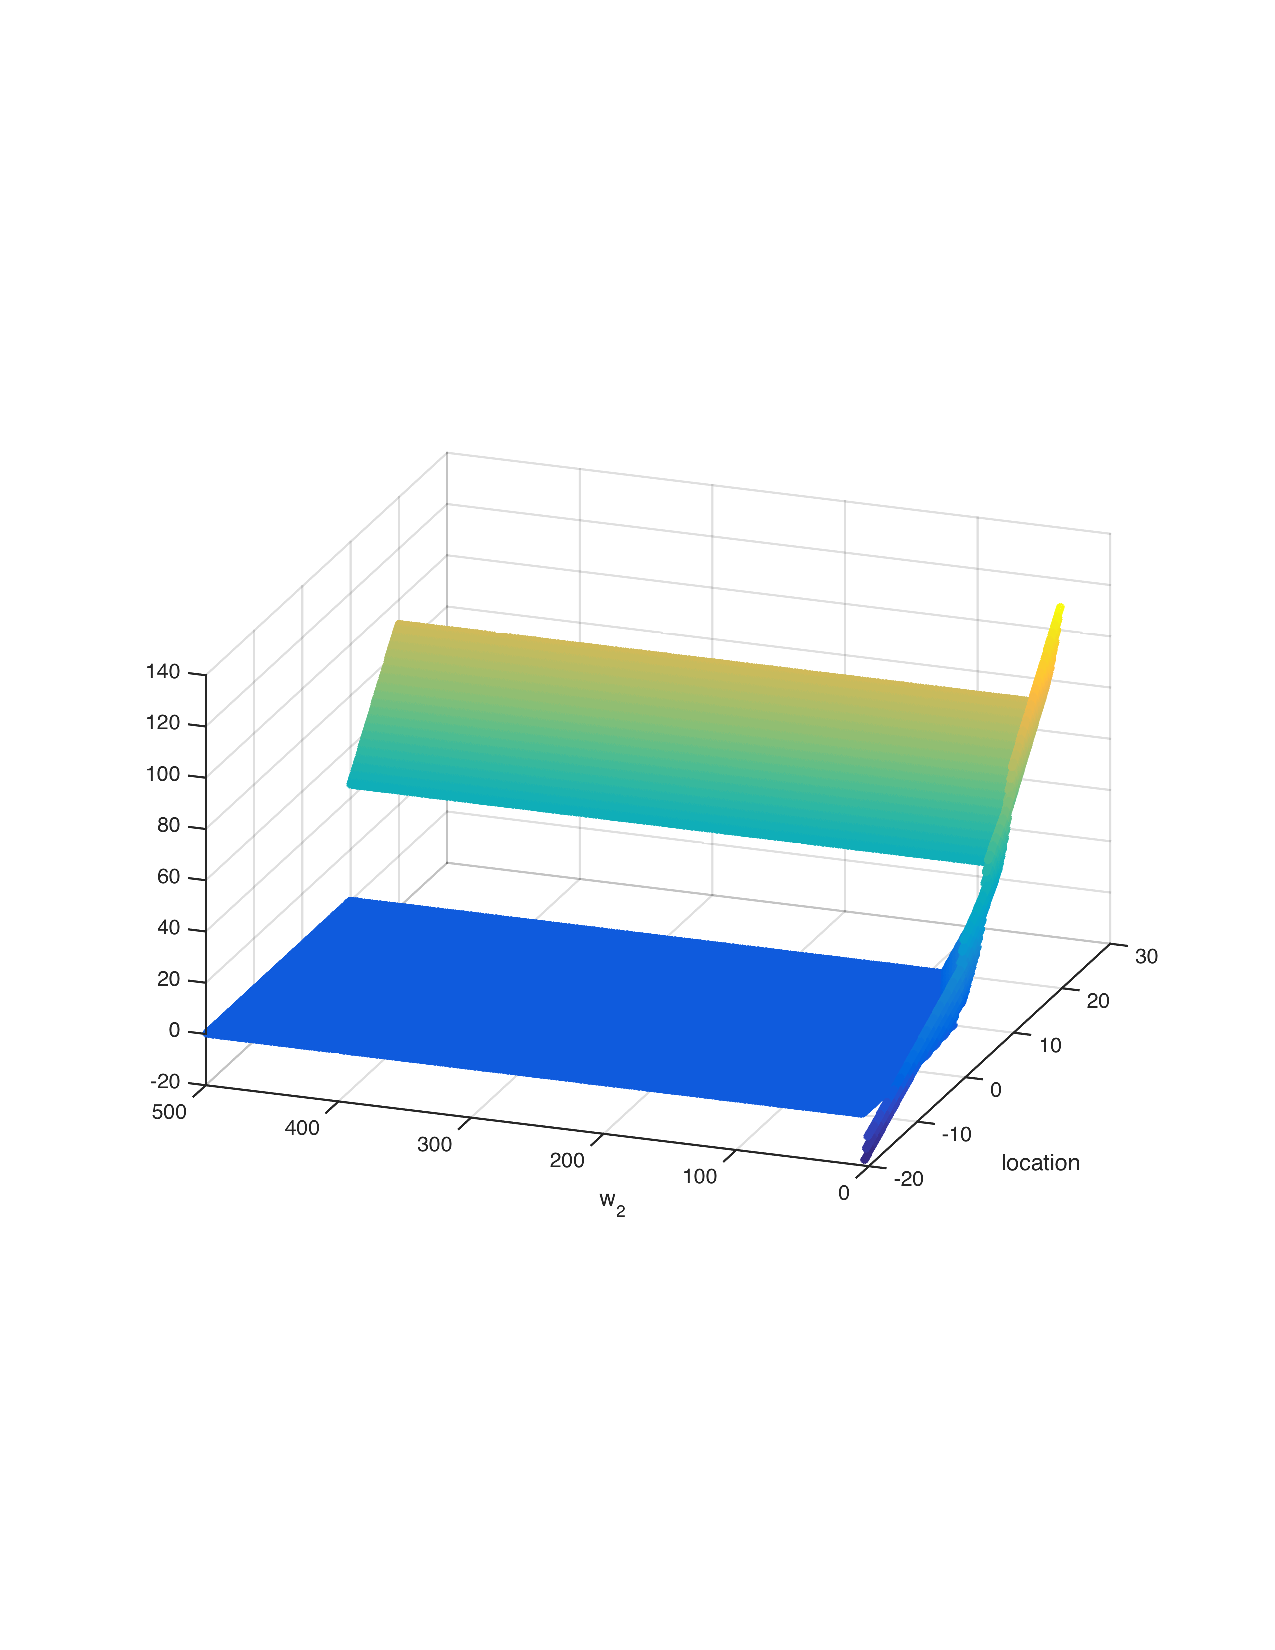
\includegraphics[width=0.8\linewidth, height=0.55\linewidth]{images/robot1d}
    \caption{The optimal value function for the multi-objective navigation domain. The vehicle incurs a movement cost at lower values of {\footnotesize $w_2$} when it is located near the {\footnotesize $ \mathtt{threshold} $}.}
    \label{fig:vehicle1d}            
\end{figure}
%------------------------------------------------------------------------------

\subsection{Influenza Public Health Policy}
\label{sec:results_influenza}

Influenza viruses continuously challenge human hosts with new variants and cause complex epidemics. Compartmental models are a widely used modelling technique within epidemiology to investigate the spread of infection diseases. In this domain we investigate the sensitivity of two different Influenza models to an infection rate parameter {\footnotesize $ \eta \in [0.0, 1.0]$}. 

The common components of both models can be defined as:
\begin{itemize}
    \item {\footnotesize $ \Action \in \left\lbrace 0, 0.25, 0.50, 1.0 \right\rbrace $} is the proportion to vaccinate 
    \item {\footnotesize $ \Reward\left(\vec{w}, cost_{\mathtt{inf}}, cost_{\mathtt{vaccine}}, s, i, a \right) = w_1 \cdot \Reward_{\mathtt{inf}} + w_2 \cdot \Reward_{\mathtt{vaccine}}$} where, \\
    {\footnotesize 
        \abovedisplayskip=10pt
        \belowdisplayskip=0pt
        \renewcommand{\arraystretch}{1.5}
        \begin{tabular}{ll}    
            $ \Reward_{\mathtt{inf}}(i, cost_{\mathtt{inf}}) = $ &  $ $ \\
            \qquad $ \begin{cases}
            (i \geq 0) : & -cost_{\mathtt{inf}} \cdot i \\
            \text{otherwise} : & 0 \\
            \end{cases} $ & $ $ \\
            $ \Reward_{\mathtt{vaccine}}(s, a, cost_{\mathtt{vaccine}}) = $ &  $ $ \\
            \qquad $ \begin{cases}
            (s \geq 0) : & -cost_{\mathtt{vaccine}} \cdot s \cdot a \\
            \text{otherwise} : & 0 \\
            \end{cases} $ & $ $ \\
        \end{tabular}
    } \\
{\footnotesize $ cost_{\mathtt{inf}} $} is the incident cost of infection, akin to a burden of disease, and {\footnotesize $ cost_{\mathtt{vaccine}} $} is the unit cost of vaccination. \\    
\end{itemize}

\subsubsection{S-I Model}
\label{sec:results_influenza_sd}

A simple epidemiological model is the two compartment S-I, model where {\footnotesize $ s_t $} refers to the number of susceptibles and {\footnotesize $ i_t $} to the number of infected in the population at time {\footnotesize $ t $}. At each time step the sub-populations are updated according to the following equations:
{\footnotesize
\begin{align*}
    s_{t + 1} &= - s_t \cdot ( \eta + a ) \\
    i_{t+1} &= \eta \cdot s_t 
\end{align*}
}
where {\footnotesize $ \eta \in [0, 1]$} is the rate of infection and {\footnotesize $ a_t \in \left\lbrace 0, \ldots, 1.0\right\rbrace $} is the proportion of susceptibles {\footnotesize $ s_t $} to be vaccinated. The S-I model can be formulated as PHMDP as follows:
\begin{itemize}
    \item {\footnotesize $ \State = \left\langle s, i \right\rangle$}, where $ s $ and $ i $ are as defined above
    \item The transition function {\footnotesize \Transition} for each state variable in {\footnotesize \State} is given by:    \\
    {\footnotesize 
        \abovedisplayskip=5pt
        \belowdisplayskip=0pt
        \renewcommand{\arraystretch}{1.5}
        \begin{tabular}{ll}
            $ \Transition\left( s' | s, i, a \right) =$ & $ \delta \left[ s' - (- s \cdot (\eta + a)) \right] $ \\
            $ \Transition\left( i' | s, i, a \right) =$ & $ \delta \left[ i' - (\eta \cdot s) \right] $ \\
        \end{tabular}
    }%
\end{itemize} 

\subsubsection{S-I-R-S Model}
\label{sec:results_influenza_sirs}

A more complex epidemiological model is the three compartment S-I-R-S, model where {\footnotesize $ s_t $} refers to the number of susceptibles, {\footnotesize $ i_t $} to number of infected and {\footnotesize $ r_t $} to the recovered in the population at time {\footnotesize $ t $}. At each time step the sub-populations are updated according to the following equations:
{\footnotesize
\begin{align*}
    s_{t + 1} &= -\eta \cdot s_t \cdot i_t + \lambda \cdot r_t - a_t \cdot s_t \\
    i_{t + 1} &= \eta \cdot s_t \cdot i_t - \beta \cdot i_t \\
    r_{t+1} &= \beta \cdot i_t - \lambda \cdot r_t 
    %    d_{t+1} &= e \cdot i_t 
\end{align*}
}
where {\footnotesize $ \eta \in [0, 1]$} is the rate of infection, {\footnotesize $ \beta \in [0, 1]$} is the rate of recovery and {\footnotesize $ \lambda \in [0, 1]$} is the rate of susceptibility, and {\footnotesize $ a_t \in \left\lbrace 0, \ldots, 1.0\right\rbrace $} is the proportion of susceptibles {\footnotesize $ s_t $} to be vaccinated. The S-I-R-S model can be formulated as PHMDP as follows:
\begin{itemize}
    \item {\footnotesize $ \State = \left\langle s, i, r \right\rangle$}, where $ s $, $ i $, and $ r $ are as defined above
    \item The transition function {\footnotesize \Transition} for each state variable in {\footnotesize \State} is given by:    \\
    {\footnotesize 
        \abovedisplayskip=5pt
        \belowdisplayskip=0pt
        \renewcommand{\arraystretch}{1.5}
        \begin{tabular}{ll}
            $ \Transition\left( s' | s, i, r, a \right) =$ & $ \delta \left[ s' - (- \eta \cdot s \cdot i + \lambda \cdot r -a \cdot s) \right] $ \\
            $ \Transition\left( i' | s, i, r, a \right) =$ & $ \delta \left[ i' - (\eta \cdot s \cdot i - \beta \cdot i) \right] $ \\
            $ \Transition\left( r' | s, i, r, a \right) =$ & $ \delta \left[ r' - (\beta \cdot i - \lambda \cdot r) \right] $ \\            
        \end{tabular}
    }%
\end{itemize} 

Figures~\ref{fig:influenza_sd} shows the effect of the infection rate parameter {\footnotesize $\eta$} on the susceptible populations under both the S-I and S-I-R-S model specifications. The parameters of the models were set to {\footnotesize$ \beta = 0.27, \lambda = 0.23, cost_{\mathtt{inf}} = 95.0$} and {\footnotesize$cost_{\mathtt{vaccine}} = 33.0$}. Upon comparing Figures~\ref{fig:influenza_sd_value_function}
and~\ref{fig:influenza_sirs_value_function} we can see that the deleterious affects of increasing {\footnotesize $\eta$} are evident earlier and is more stable in the S-I model. The affect of {\footnotesize $\eta$} in the S-I-R-S model is only evident at higher values of {\footnotesize $s$}, where the affect is dramatic. The differences between both models is due the deleterious affect of an increasing {\footnotesize $ \eta $} being counteracted by the amount of individuals becoming susceptible due to the rate of susceptibility {\footnotesize $ \lambda $}. The \textit{sensitivity} of both model specifications, shown in Figure~\ref{fig:influenza_sirs}, further illustrates the affect of {\footnotesize $\eta$} on {\footnotesize $s$} in both models. 

%------------------------------------------------------------------------------
% Figure
\begin{figure}[h!]
    \centering
    \begin{subfigure}[b]{0.5\textwidth}    
        \centering
        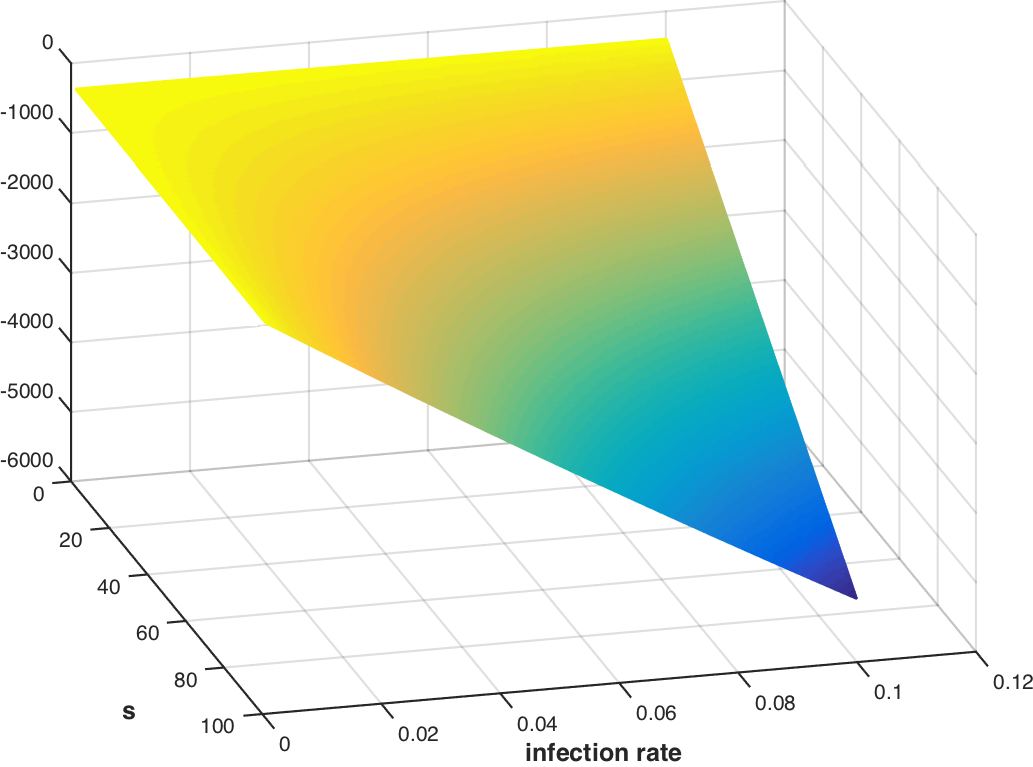
\includegraphics[width=0.8\linewidth, height=0.55\linewidth]{images/sd_infection_s}
        \caption{S-I model.}
        \label{fig:influenza_sd_value_function}
        \vspace{1em}
    \end{subfigure}  
    \begin{subfigure}[b]{0.5\textwidth}    
        \centering
        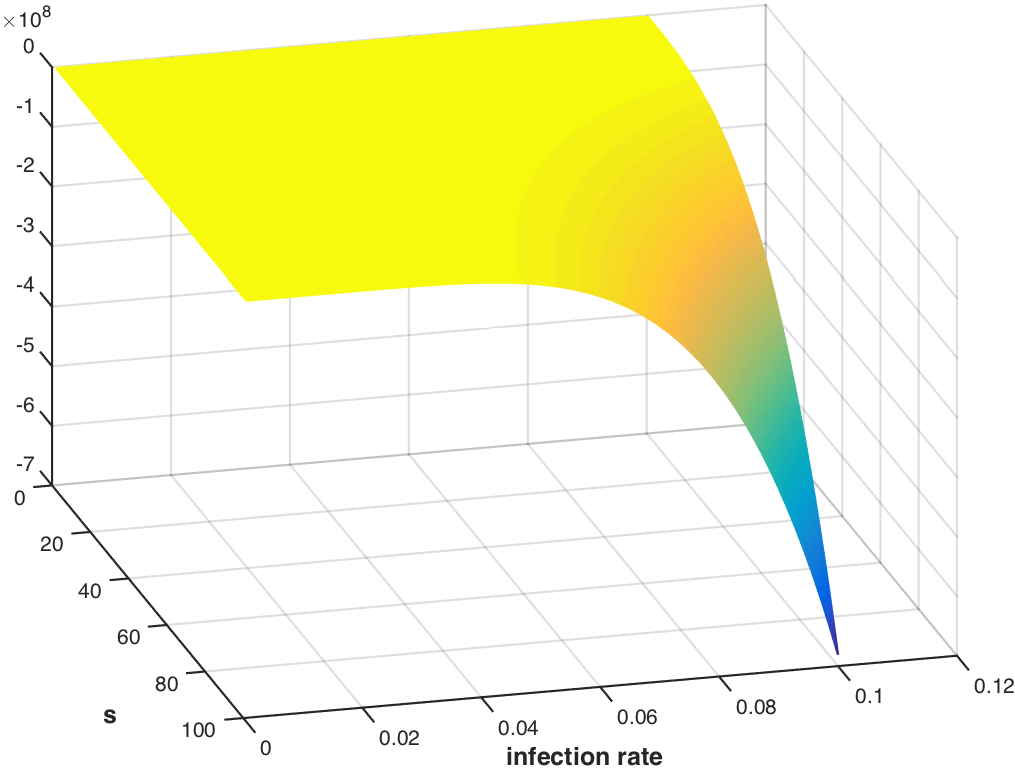
\includegraphics[width=0.8\linewidth, height=0.55\linewidth]{images/sir_infection_s}
        \caption{S-I-R-S model.}
        \label{fig:influenza_sirs_value_function}
        \vspace{1em}
       \end{subfigure}         
    \caption{The effect of the infection rate {\footnotesize $\eta$} on the number of susceptibles {\footnotesize $s$} under different Influenza model specifications.}
    \label{fig:influenza_sd}    
\end{figure}
%------------------------------------------------------------------------------

%------------------------------------------------------------------------------
% Figure
\begin{figure}[t!]
    \centering
    \begin{subfigure}[b]{0.5\textwidth}    
        \centering
        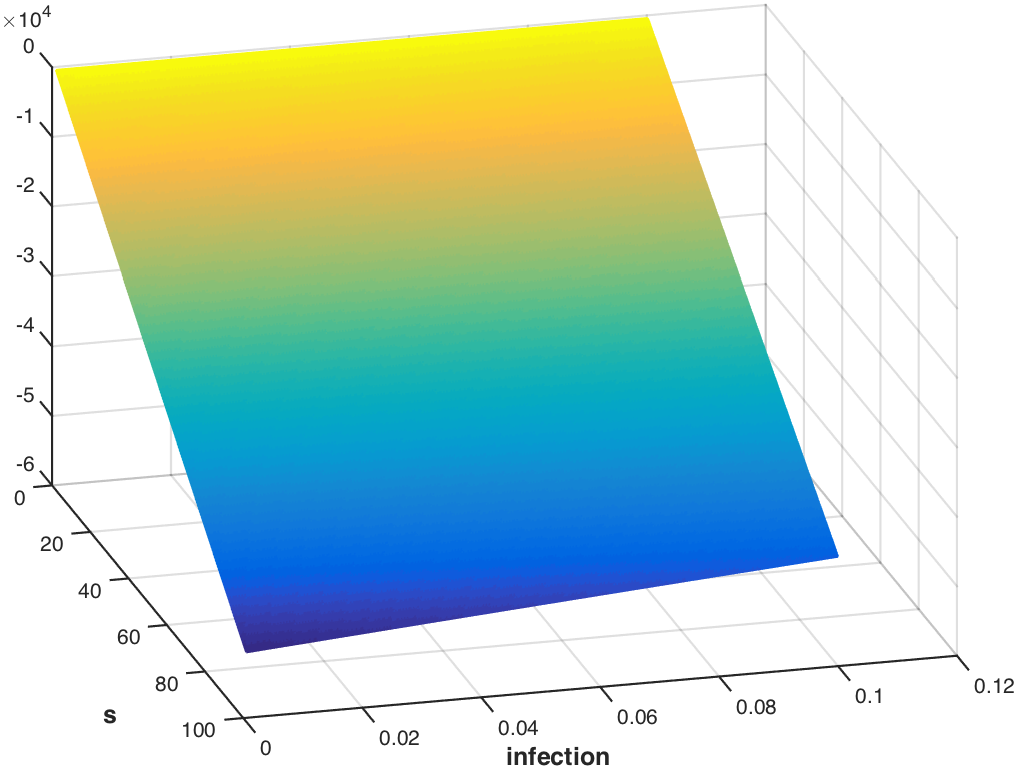
\includegraphics[width=0.8\linewidth, height=0.55\linewidth]{images/sd_infection_sensitivity}
        \caption{S-I model.}
        \label{fig:influenza_sd_sensitivity}
    \end{subfigure}  
    \begin{subfigure}[b]{0.5\textwidth}    
        \centering
        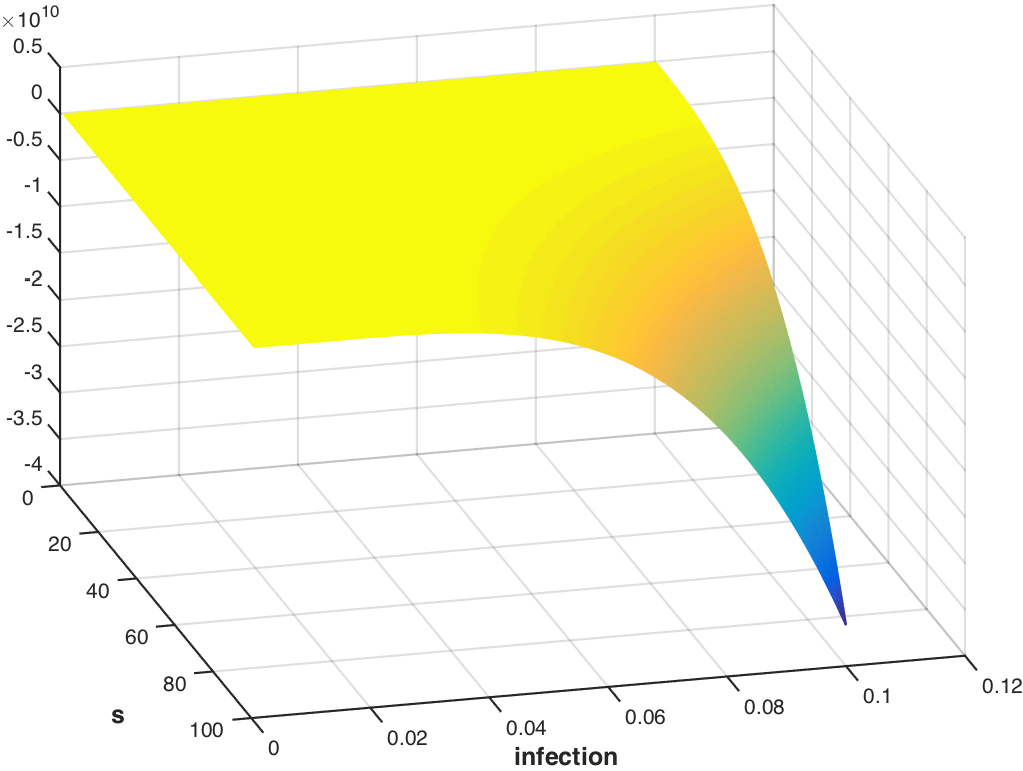
\includegraphics[width=0.8\linewidth, height=0.55\linewidth]{images/sir_infection_sensitivity}
        \caption{S-I-R-S model.}
        \label{fig:influenza_sirs_sensitivity}
    \end{subfigure}  
    \caption{The sensitivity of the number of susceptibles {\footnotesize $s$} to changes in the infection rate {\footnotesize $\eta$} under different Influenza model specifications.}
    \label{fig:influenza_sirs}      
\end{figure}
%------------------------------------------------------------------------------

\subsection{Optimal Execution}
\label{sec:results_oe}

Institutional investors often need to acquire or liquidate a number of shares within a given period of time. Indirect transaction costs are an important consideration for institutional investors who often want to transact a number of shares that exceeds the available liquidity i.e. there may not be a counterparty or counterparties that wish to take the other side of the trade at the same volume. There is a clear trade-off between the market impact of transacting immediately and the volatility of slow execution. 

In this domain we use a price impact model inspired by Bertsimas and Lo~\parencite{Bertsimas_JFM_1998} to investigate the optimisation of parameters within a static parameterized proportional liquidation policy, where the investor can vary the proportion of remaining inventory to sell. The optimal execution domain can be defined as:
\begin{itemize}
    \item {\footnotesize $ \State = \left\langle price, inv \right\rangle$}, where $ price $ is the price of the asset and $ inv $ is the inventory remaining
    \item The transition function {\footnotesize \Transition} for each state variable in {\footnotesize \State} is given by:    \\
    {\footnotesize 
        \abovedisplayskip=5pt
        \belowdisplayskip=0pt
        \renewcommand{\arraystretch}{1.5}
        \begin{tabular}{ll}
            $ \Transition\left( price' | price, inv, a \right) =$ & $ \delta \left[ price' - (price + \kappa + \sigma \cdot \epsilon) \right] $ \\
            $\Transition\left( inv' | price, inv, n \right) =$ & $ \delta \left[ inv' - (inv - inv \cdot a) \right] $ \\
        \end{tabular}
    }%
%    \item {\footnotesize $ \Action \in \left\lbrace 0, 0.25, 0.50, 1.0 \right\rbrace $} is the proportion of the remaining inventory to sell    
    \item {\footnotesize $ \Reward\left(price, price_0, inv, a \right) =$} \\
    {\footnotesize 
        \abovedisplayskip=10pt
        \belowdisplayskip=0pt
        \renewcommand{\arraystretch}{1.5}
        \begin{tabular}{ll}    
           $ \begin{cases}
                (inv \geq a) : & a \cdot inv \cdot price - inv \cdot price_0 \\
                \text{otherwise} : & 0 \\
            \end{cases} $ & $ $ \\
        \end{tabular}
    } \\    
\end{itemize}

The investor aims to minimise \textit{price slippage}, which is defined as the difference between the theoretical benchmark price and the actual price received.

%\subsubsection{Constant Liquidation Policy}
%\label{sec:results_oe_constant}
%
%With a constant liquidation policy the investor chooses to sell a constant number of assets at each time period. This specific scenario is defined by the following:
%\begin{itemize}
%    \item {\footnotesize 
%         \begin{tabular}{ll}
%            $ \Transition\left( inv' | price, inv, a \right) = $ & $ $ \\
%            $ \qquad \delta \left[ inv' - \begin{cases}
%            inv \geq a : & inv - a \\
%            \text{otherwise} : & inv \\
%            \end{cases} \right] $ & $ $\\
%        \end{tabular}
%    }%
%    \item {\footnotesize $ \Reward\left(price, price_0, inv, a \right) =
%        \begin{cases}
%            (inv \geq a) : & a \cdot price - a \cdot price_0 \\
%            \text{otherwise} : & 0 \\
%        \end{cases} $}
%    \item {\footnotesize $ \Action \in \left\lbrace 0, \ldots, inv_0 \right\rbrace $} is the number of the remaining inventory to sell    
%\end{itemize}

%\subsubsection{Fractional Liquidation Policy}
%\label{sec:results_or_proportional}
%
%With a proportional liquidation policy the investor chooses to sell a constant proportion of assets at each time period. This specific scenario is defined by the following:
%\begin{itemize}
%    \item {\footnotesize $\Transition\left( inv' | price, inv, n \right) = \delta \left[ inv' - (inv - inv \cdot a) \right] $}
%    \item {\footnotesize $ \Reward\left(price, price_0, inv, a \right) =
%        \begin{cases}
%        (inv \geq a) : & a \cdot inv \cdot price - inv \cdot price_0 \\
%        \text{otherwise} : & 0 \\
%        \end{cases} $} 
%    \item {\footnotesize $ \Action \in \left\lbrace 0, 0.25, 0.50, 1.0 \right\rbrace $} is the proportion of the remaining inventory to sell    
%\end{itemize}

Figure~\ref{fig:opt_execution} displays the optimal {\footnotesize$ \Horizon = 5 $} value function under the parameterized proportional liquidation policy. The parameters of the models were set to {\footnotesize$ \kappa = 1.65 \times 10^{-3}, price_0 = 10.0, price = 20.0$} and {\footnotesize $inv = \left\lbrace 0.0, 200.0\right\rbrace$}. The surface of the function shows that for high inventory {\footnotesize $inv$}, increasing the policy parameter from {\footnotesize $ 0.0 $} to {\footnotesize $ 1.0 $}, results in an increased reward by limiting exposure to price slippage.

%------------------------------------------------------------------------------
% Figure
\begin{figure}[h!]
    \centering
    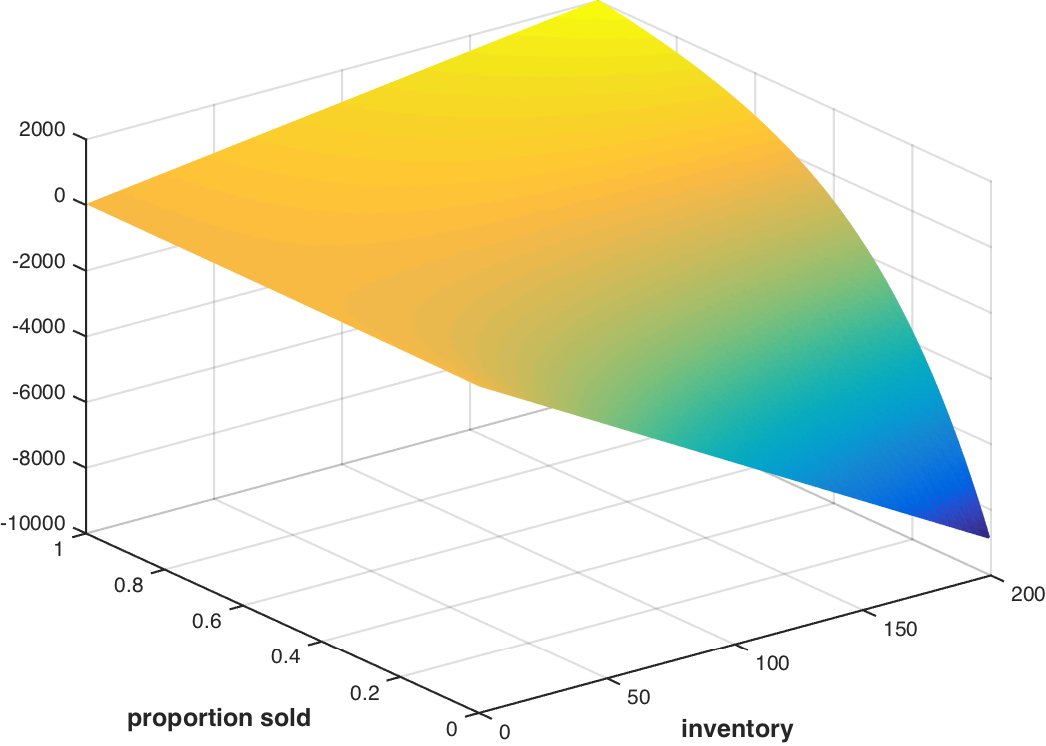
\includegraphics[width=0.8\linewidth, height=0.55\linewidth]{images/opt_execution_fraction}
    \caption{The optimal execution value function under the parameterized proportional liquidation policy. The reward obtained is maximised by increasing the policy parameter (proportion sold) over all levels of inventory.}
    \label{fig:opt_execution}            
\end{figure}
%------------------------------------------------------------------------------

%------------------------------------------------------------------------------
% Figure
%\begin{figure}[t!]
%    \centering
%%    \begin{subfigure}[b]{0.5\textwidth}    
%%%        \centering
%%        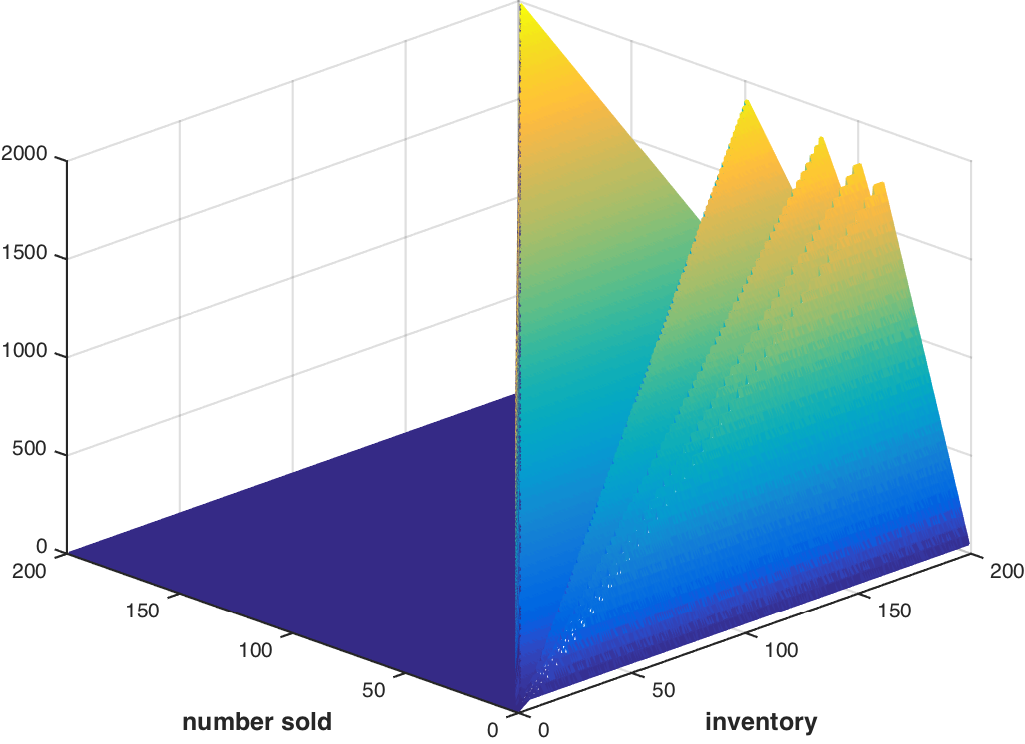
\includegraphics[width=0.8\linewidth, height=0.55\linewidth]{images/opt_execution_budget}
%%        \caption{Constant liquidation.}
%%        \label{fig:opt_execution_w1}
%%        \vspace{1em}
%%    \end{subfigure}
%    
%    \begin{subfigure}[b]{0.5\textwidth}    
%%        \centering
%        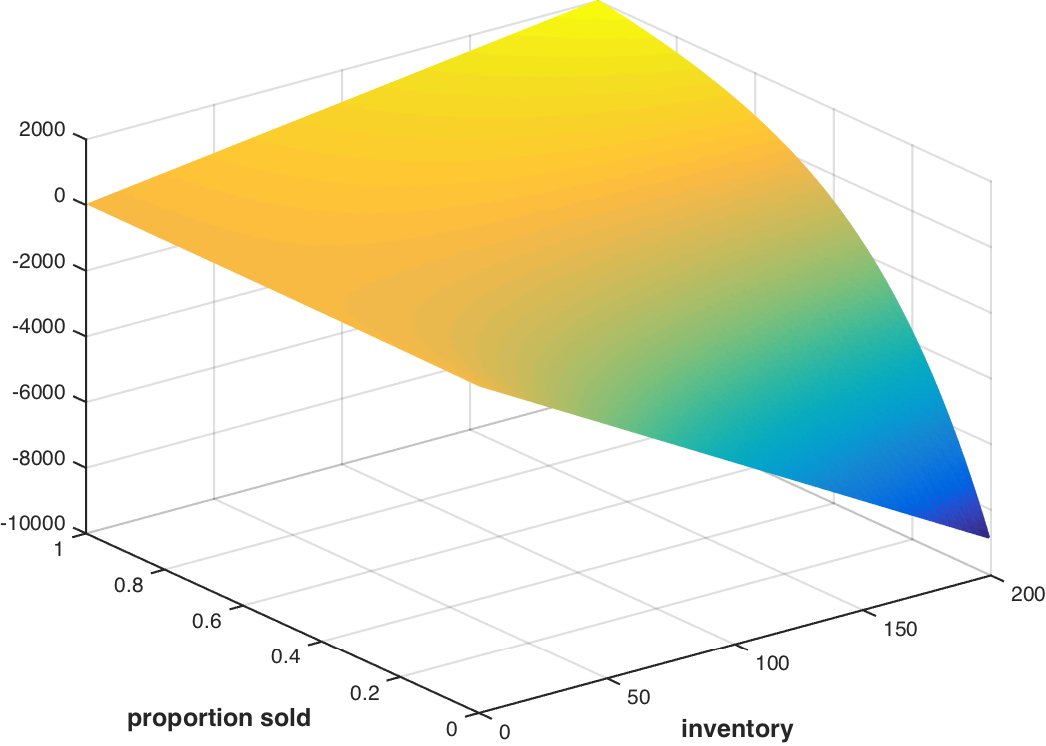
\includegraphics[width=0.8\linewidth, height=0.55\linewidth]{images/opt_execution_fraction}
%%        \caption{Fractional liquidation.}
%        \label{fig:opt_execution_w2}
%    \end{subfigure}  
%    \caption{The optimal execution value function under the proportional liquidation policy.}
%    \label{fig:opt_execution}
%\end{figure}
%------------------------------------------------------------------------------